% !TEX root =  master.tex
\chapter{Web Application Design}\label{ch:web-application-design}

\begin{figure}[hbtp]
    \centering
    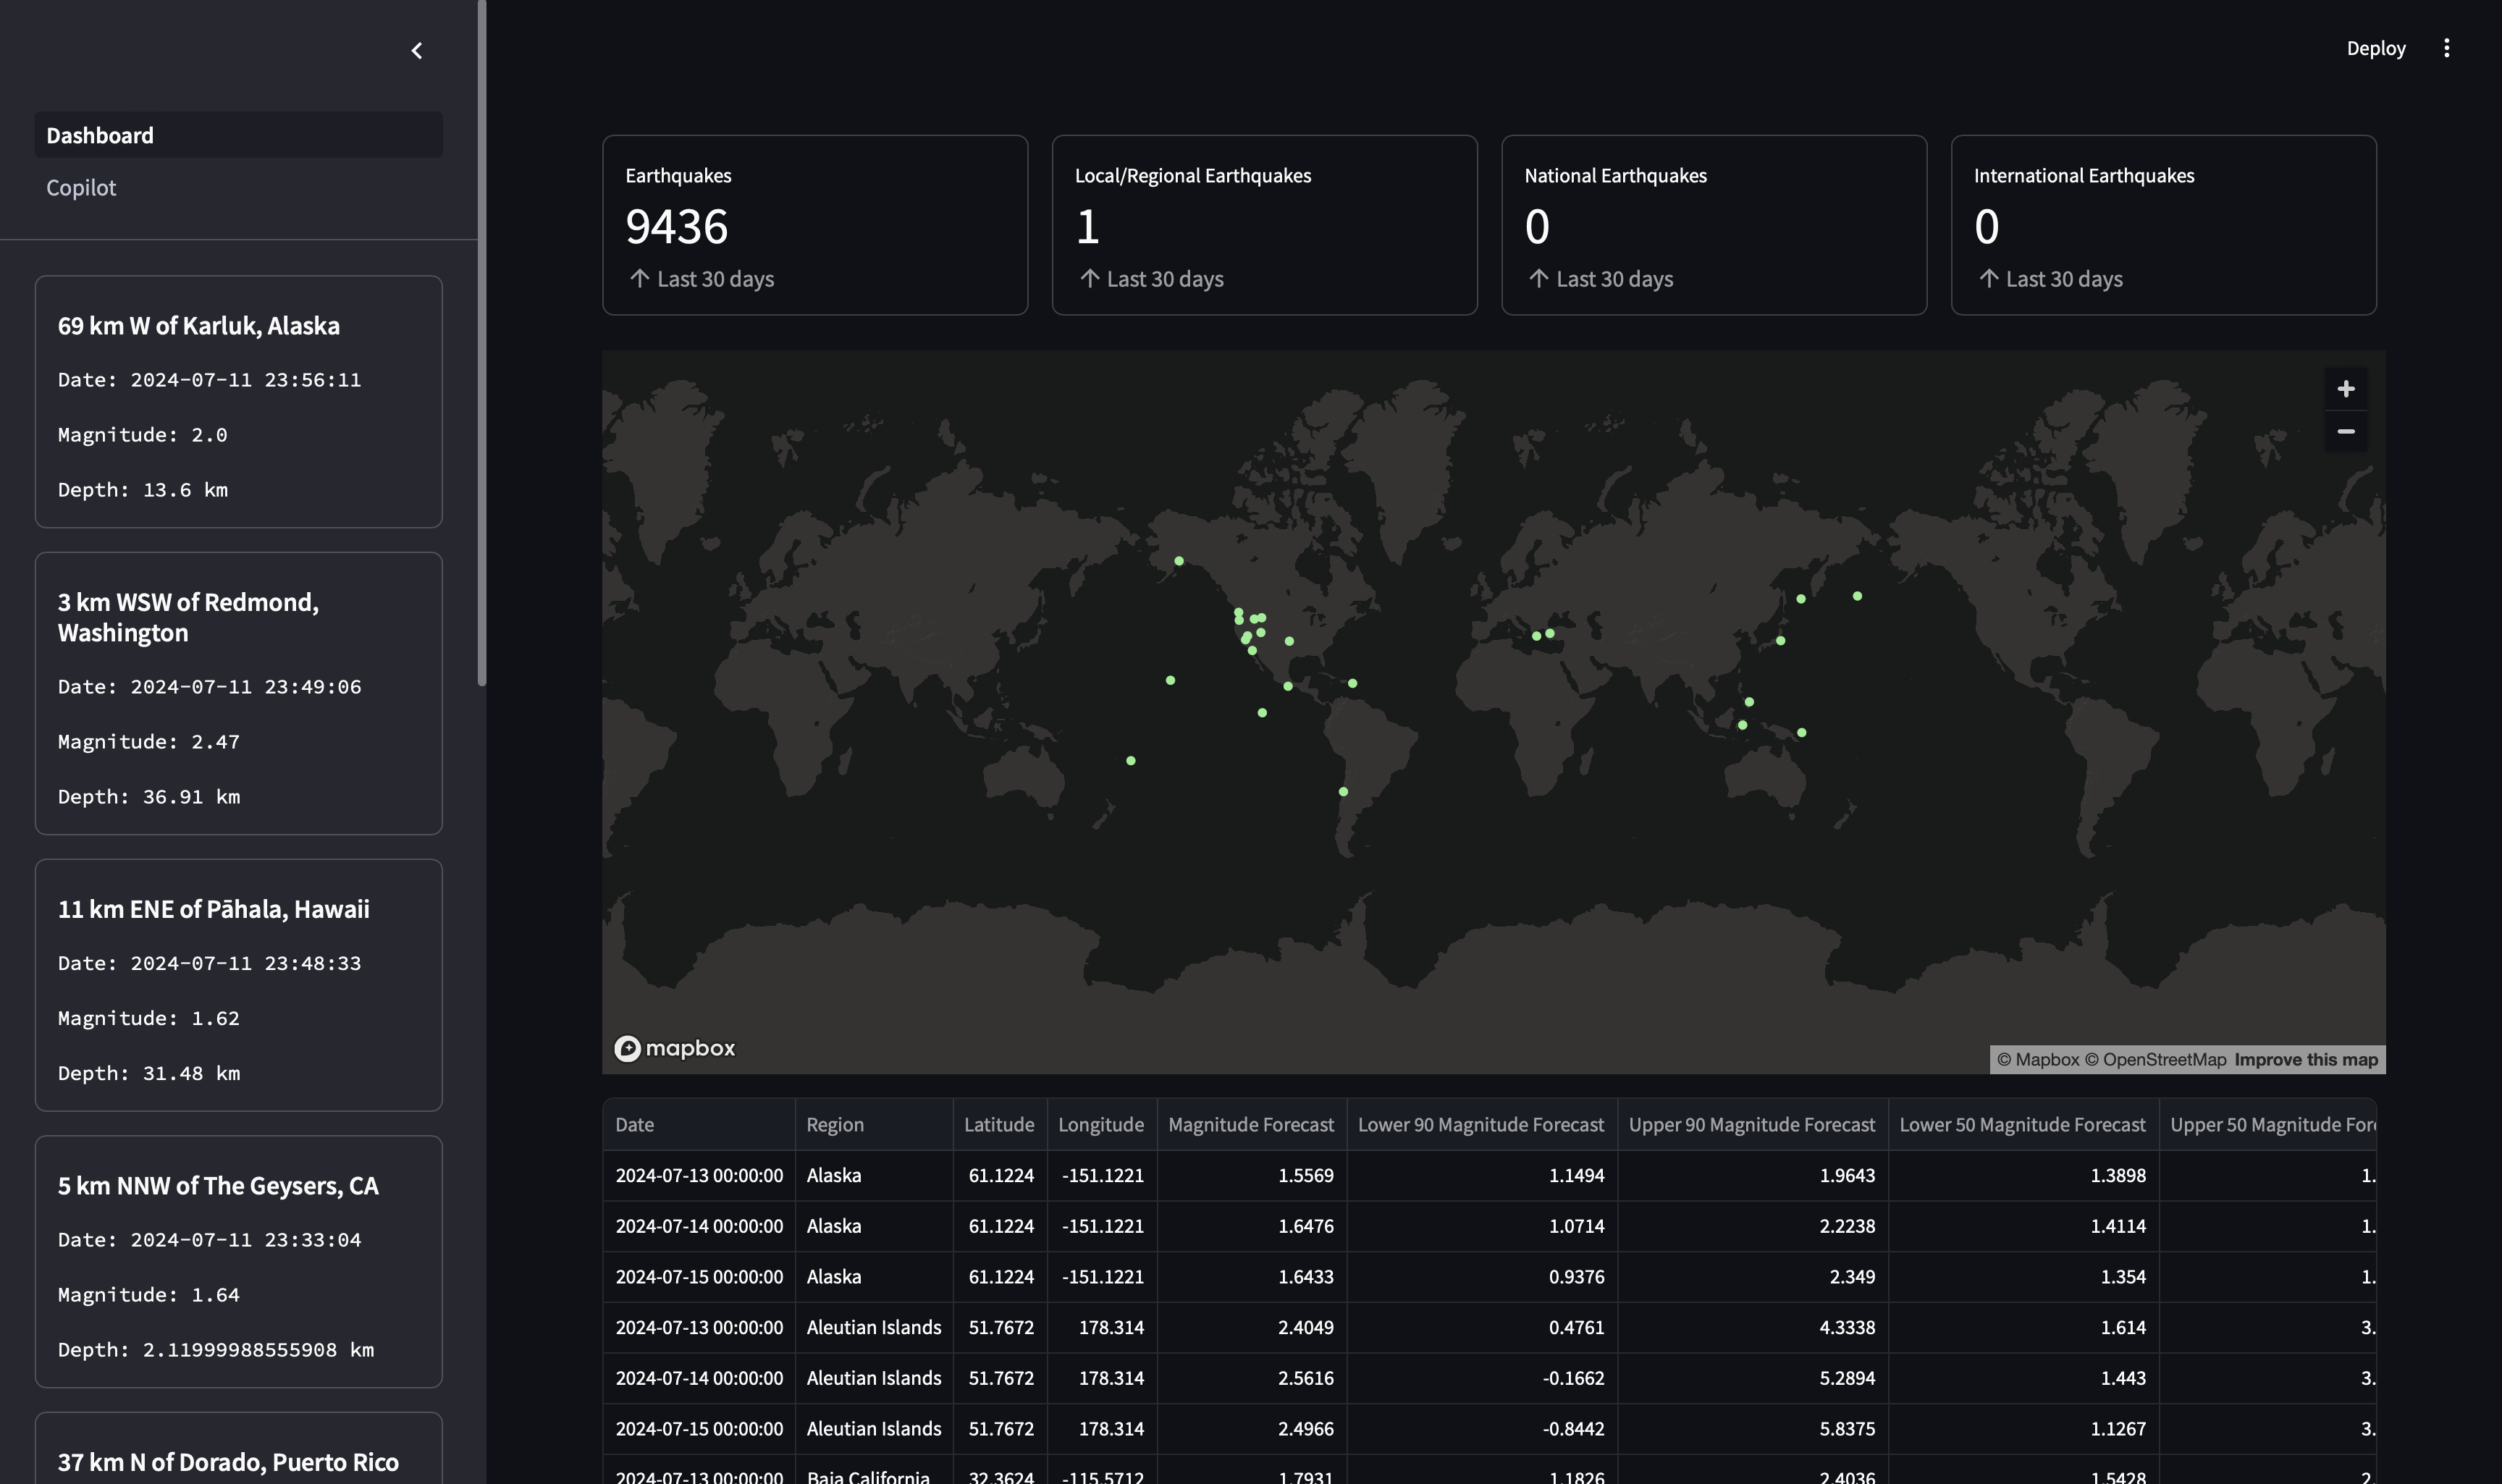
\includegraphics[scale=0.25]{img/dashboard.png}
    \captionsetup{format=hang}
    \caption{\label{fig:dashboard}Interactive dashboard displaying
        recent earthquakes, with a map featuring earthquake forecasts
        and a corresponding table detailing the forecasted values for
        magnitude and depth.}
\end{figure}

\begin{figure}[hbtp]
    \centering
    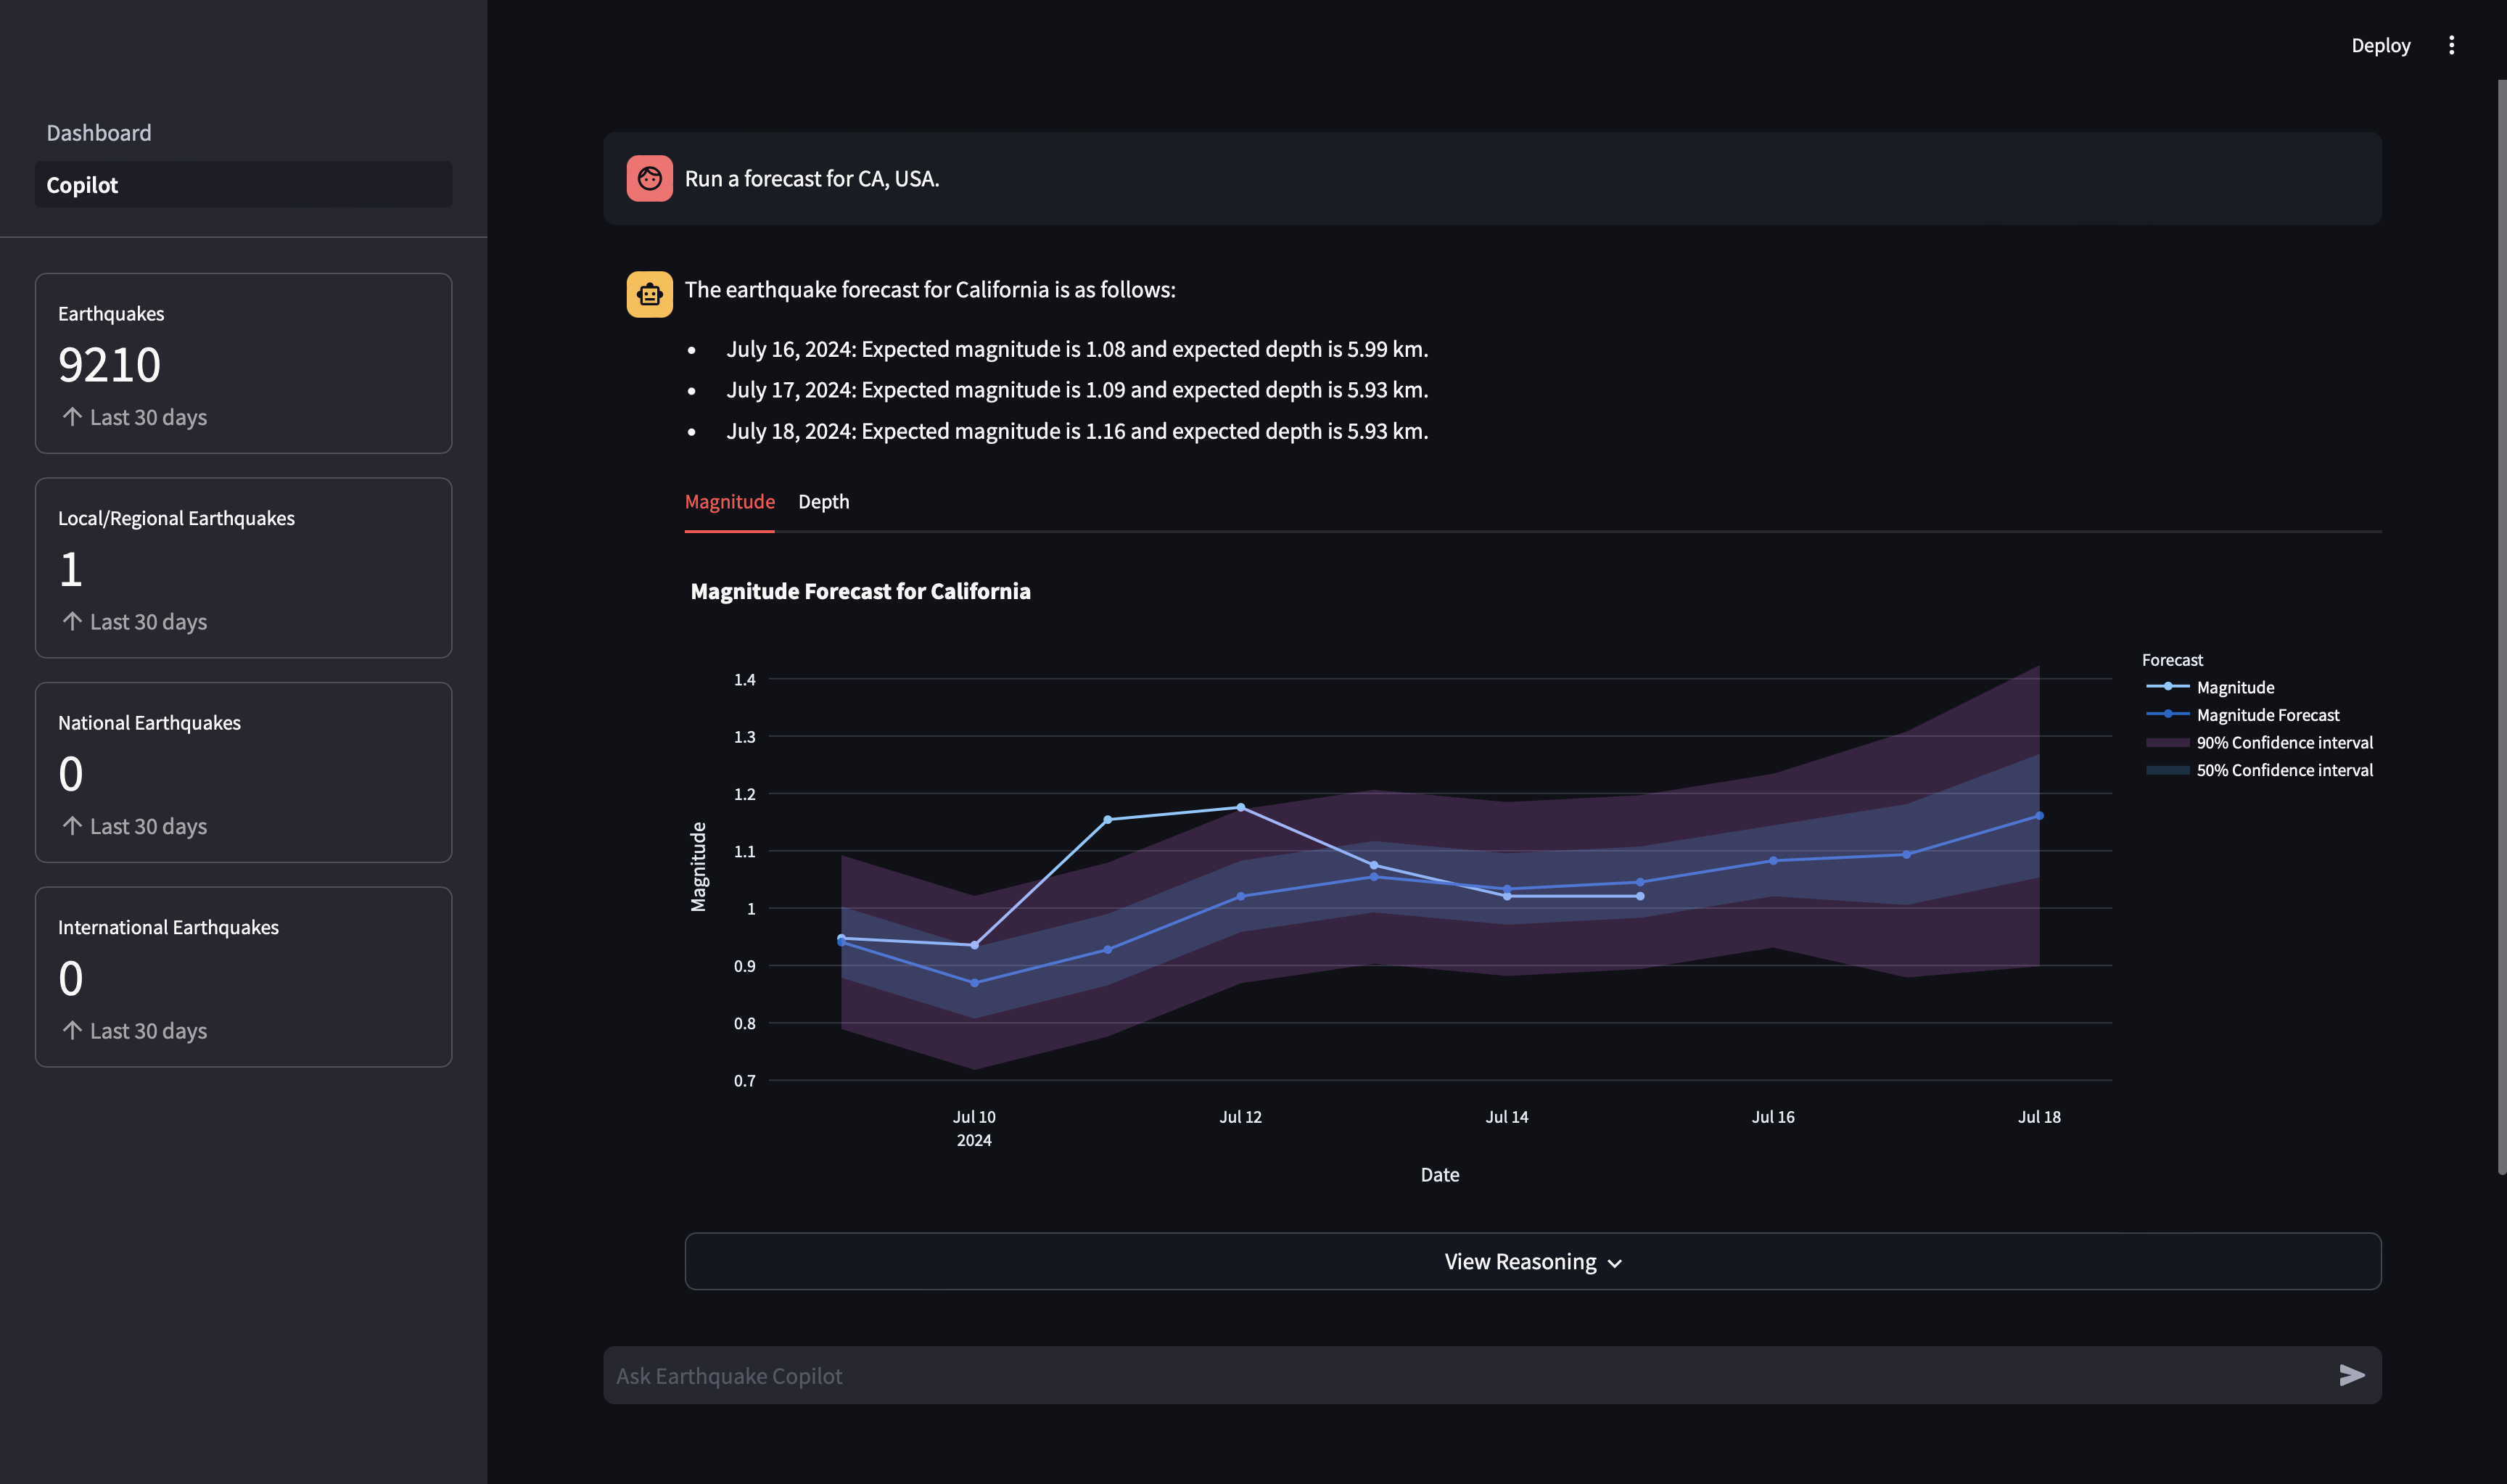
\includegraphics[scale=0.25]{img/copilot-forecast-example.png}
    \captionsetup{format=hang}
    \caption{\label{fig:copilot}Copilot interface showcasing human-AI
        collaboration, where an \ac{LLM}-powered AI agent assists by
        answering questions, running forecasts, and recommending
        precautionary actions.}
\end{figure}

\begin{figure}[hbtp]
    \centering
    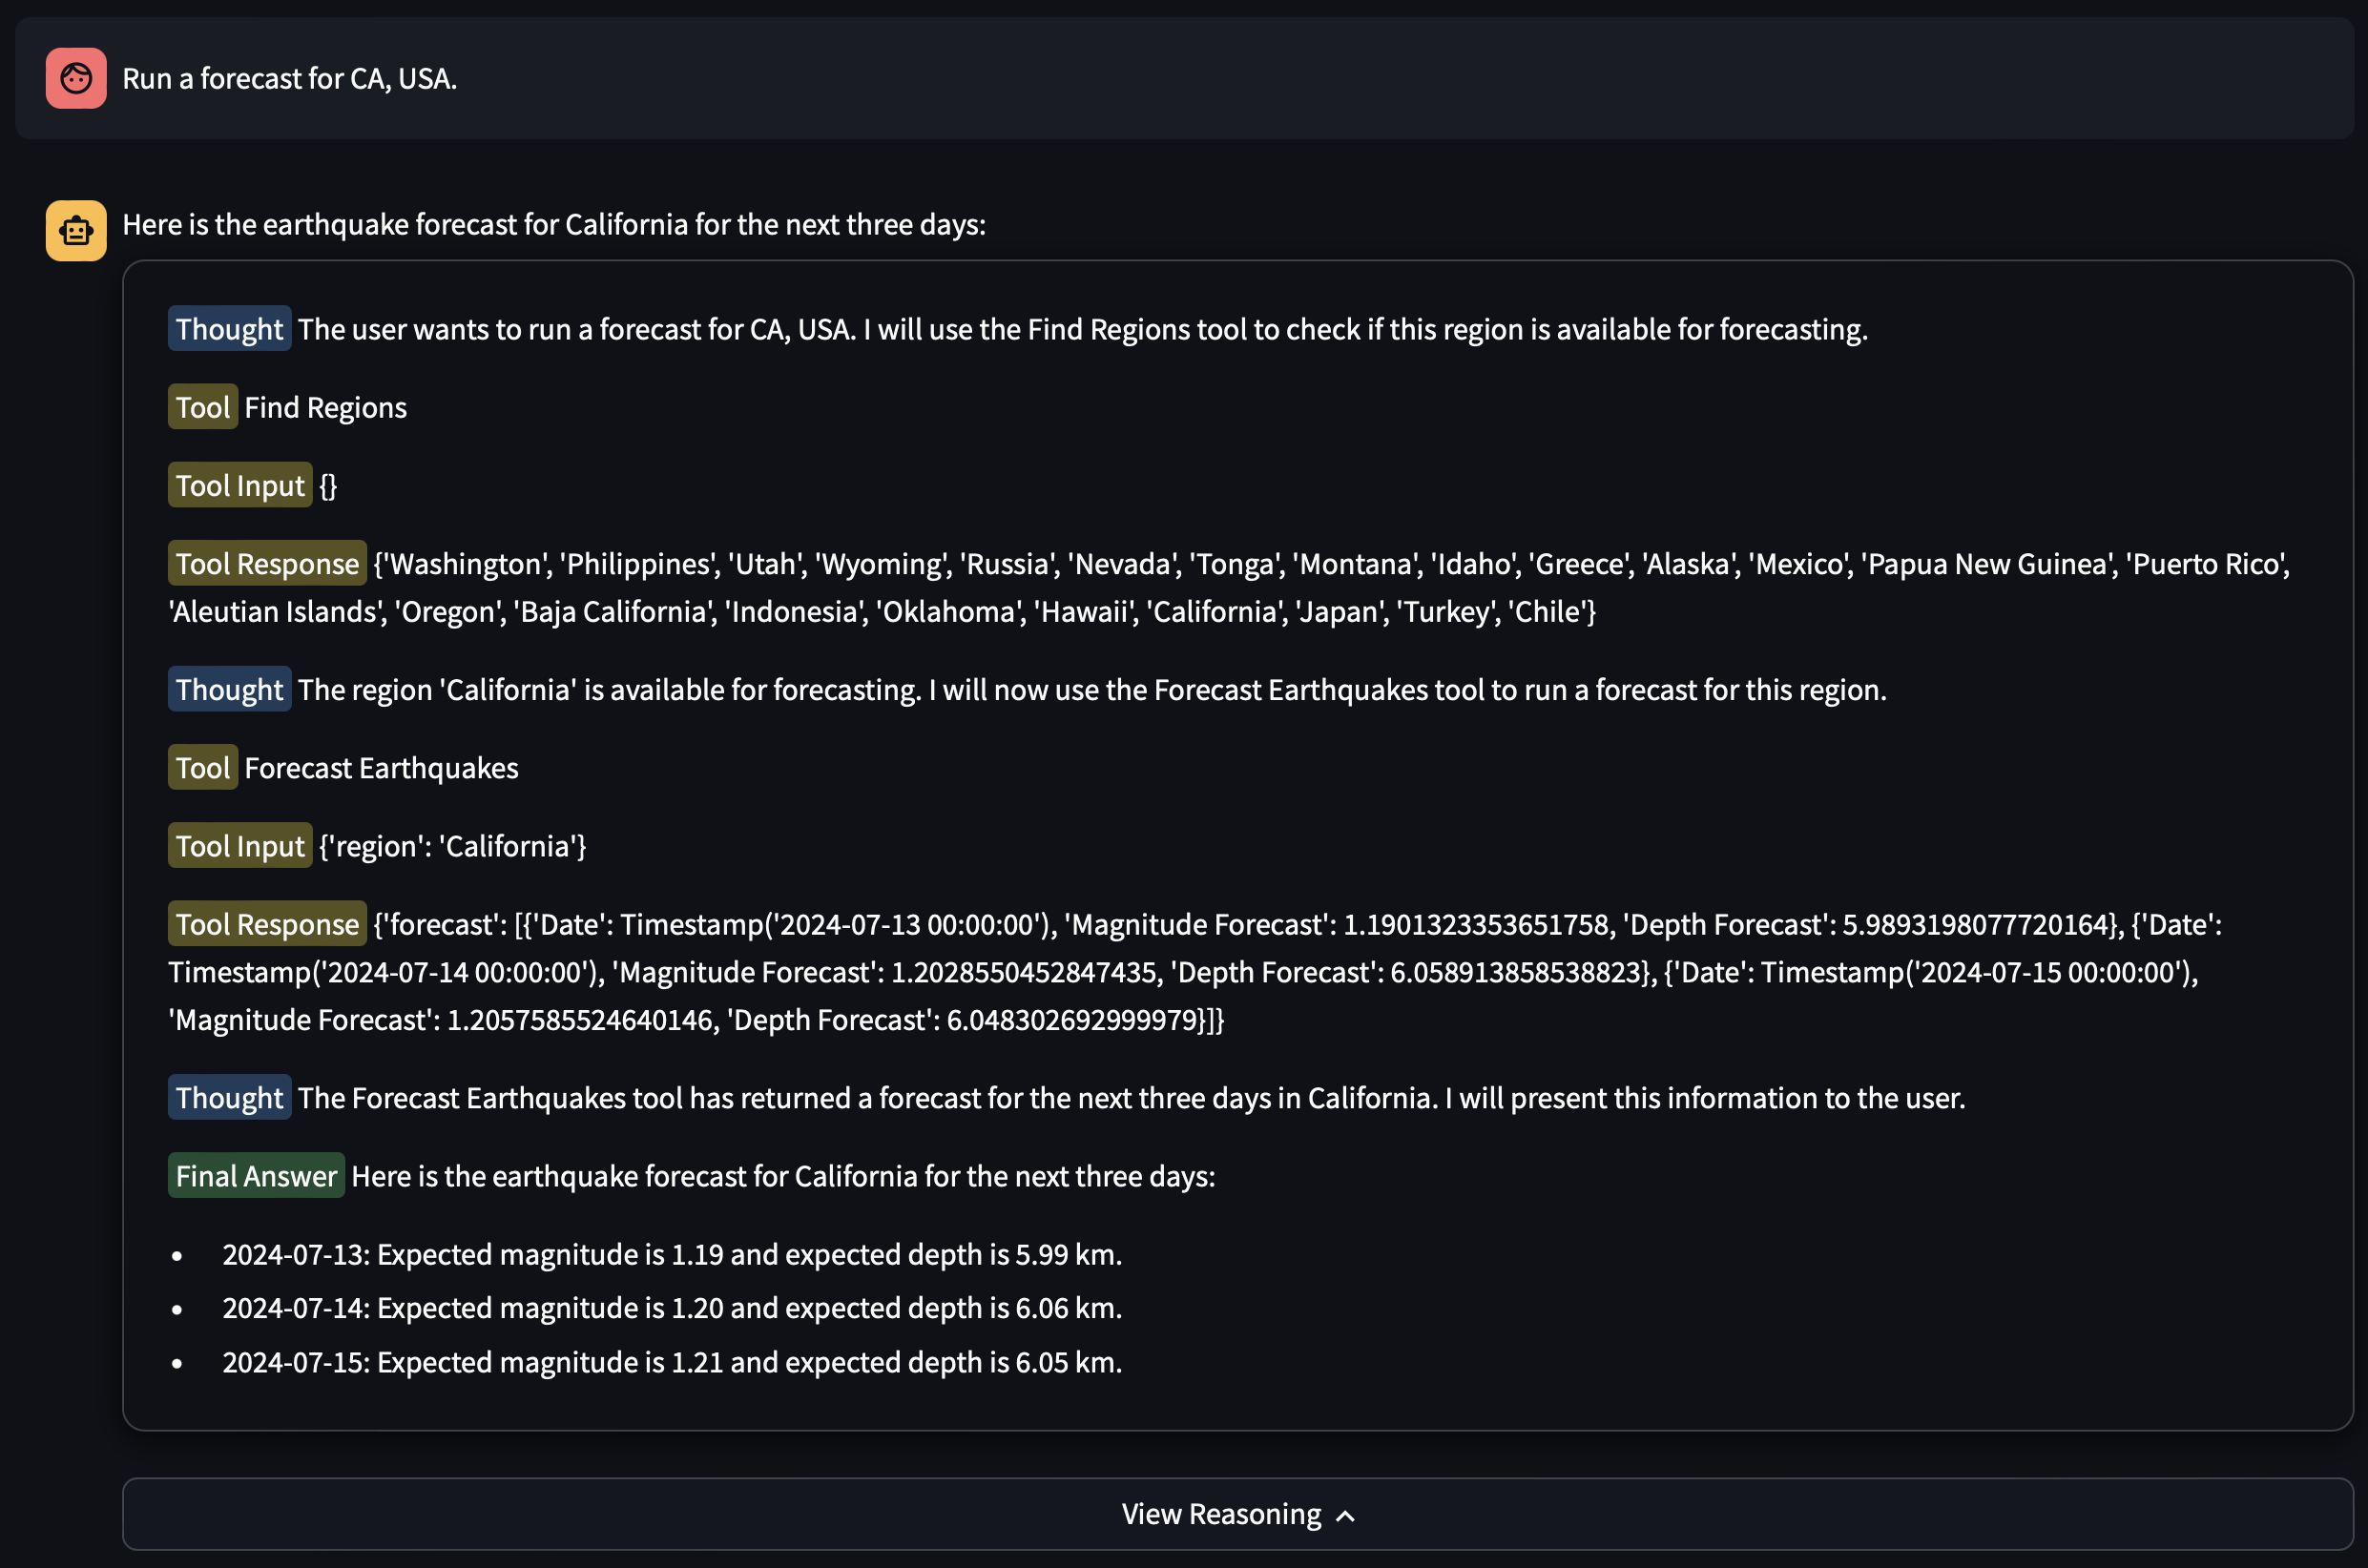
\includegraphics[scale=0.35]{img/explainable-ai-agent.png}
    \captionsetup{format=hang}
    \caption{\label{fig:explainable-ai}Explainable AI in action:
        The \ac{LLM}-powered AI agent demonstrates its reasoning process as
        it runs a forecast for California, USA. By following the
        reasoning steps, the user can verify the accuracy and
        transparency of the \ac{LLM}'s operations, thereby building trust.}
\end{figure}

